\documentclass{beamer}

\usepackage{amsmath,amssymb,amsfonts}
\usepackage{array}
\usepackage[british]{babel}
\usepackage{bbm}
\usepackage{bbold}
\usepackage{beamerthemesplit}
\usepackage[bf]{caption}
\usepackage{cite}
\usepackage{color}
\usepackage{enumerate}
\usepackage{eurosym}
\usepackage{graphicx}
\usepackage{rotating}
\usepackage{slashed}
\usepackage[utf8]{inputenc}
\usepackage{xcolor}
\usepackage{array}
\usepackage{listings}

\usepackage{pgfplots}
\pgfplotsset{compat=1.10}

% My fonts:
% ---------
\usepackage{libertine}
\usefonttheme[onlymath]{serif}

%----------------------------------------------------------------------------------------
% C++ STYLES
%----------------------------------------------------------------------------------------

\definecolor{codegreen}{rgb}{0,0.6,0}
\definecolor{codegray}{rgb}{0.5,0.5,0.5}
\definecolor{codepurple}{rgb}{0.58,0,0.82}
\definecolor{backcolour}{rgb}{0.95,0.95,0.92}
\lstdefinestyle{mystyle}{
	language=C++,
  % backgroundcolor=\color{backcolour},
  commentstyle=\color{codegreen},
  keywordstyle=\color{magenta},
  numberstyle=\tiny\color{codegray},
  stringstyle=\color{codepurple},
  basicstyle=\tiny,
  breakatwhitespace=false,
  breaklines=true,
  captionpos=b,
  keepspaces=true,
  % numbers=left,
  numbersep=5pt,
  showspaces=false,
  showstringspaces=false,
  showtabs=false,
  tabsize=2,
        keywords={var, func, extends},
}
\lstset{style=mystyle}

%----------------------------------------------------------------------------------------
% OTHER STUFF
%----------------------------------------------------------------------------------------

\DeclareMathOperator{\tr}{tr}
\makeatletter
\def\amsbb{\use@mathgroup \M@U \symAMSb}
\makeatother

\usetheme{Boadilla}

\setbeamertemplate{section in toc}[sections numbered]
\setbeamertemplate{blocks}[rounded][shadow=false]
\setbeamertemplate{itemize items}[default]
\beamertemplatenavigationsymbolsempty
\setbeamercolor{footline}{bg=black}
\setbeamertemplate{footline}{%
  \raisebox{8pt}{\makebox[\paperwidth]{\hfill\makebox[15pt]{{\tiny\insertframenumber}}\qquad}}
}

\definecolor{myred}{RGB}{176,50,50}
\definecolor{myblue}{RGB}{50,50,176}
\definecolor{mygreen}{RGB}{60,166,60}

\newcommand\blfootnote[1]{%
  \begingroup
    \renewcommand\thefootnote{}\footnote{#1}%
    \addtocounter{footnote}{-1}%
    \endgroup
}


\begin{document}

\allowdisplaybreaks[1]

\title{Lattice QCD on Intel Xeon Phi's}
\author{Peter Labus \and Martin Ueding }
  \date{Cineca \\ 2017-03-23}

  %%%%%%%%%%%%%%%%%%%%%%%%%%%%%%%%%%%%%%%%%%
  %%%   TITLE SLIDE
  %%%%%%%%%%%%%%%%%%%%%%%%%%%%%%%%%%%%%%%%%%

  \begin{frame}
    \titlepage
  \end{frame}

  %%%%%%%%%%%%%%%%%%%%%%%%%%%%%%%%%%%%%%%%%%
  %%%   SLIDE 1
  %%%%%%%%%%%%%%%%%%%%%%%%%%%%%%%%%%%%%%%%%%

  \setcounter{framenumber}{0}

  \begin{frame}
    \frametitle{LQCD \& the r\^ole of the \textit{dslash} stencil}

    \begin{itemize}
      \item  Calculate integrals of the form
        \begin{align*}
          \int \mathcal D \Phi \; f[\Phi] \, e^{-S_{QCD}[\Phi]}
        \end{align*}
        after \textit{discretising} space-time through a lattice
        \vfill

      \item Algorithmic layers of LQCD:
        \begin{enumerate}
          \item Hybrid Monte Carlo
          \item Efficient Krylov Solvers for $Mx=b$ in Molecular Dynamics
          \item BLAS linear algebra
        \end{enumerate}
        \vfill

      \item Most \textit{expensive} part:\\[1mm]
        \hspace{2mm} Matrix times Vector (very large $10^9$ squared \& very sparse),\\
        \hspace{2mm} described by (next-to) nearest-neighbour stencil
        % , called \textit{dslash}
        \vfill
    \end{itemize}

  \end{frame}

  %%%%%%%%%%%%%%%%%%%%%%%%%%%%%%%%%%%%%%%%%%
  %%%   SLIDE 2
  %%%%%%%%%%%%%%%%%%%%%%%%%%%%%%%%%%%%%%%%%%

  \begin{frame}
    \frametitle{The QPhiX library (mainly: Balint Joo, Jefferson Lab)}

    \begin{itemize}
      \item Aim: provide stencil operations for \textbf{general vector machines}
        \vfill
      \item Parallelised via QMP + OpenMP + SIMD (vector intrinsics)
        \vfill
      \item C++11 template library with external C++ code generator\\
        ($\sim25k$ lines of code + $10k$ testing \& timing)
        \vfill
      % \item Implements even-odd preconditioning, mixed precision solvers, tiling/SoA data layout, 3.5d cache blocking,
      %   gauge compression, \dots
      \item Implements
        \begin{enumerate}
          \item Wilson / Wilson-Clover \textit{dslash} stencils
          \item BLAS linear algebra
          \item Krylov Solvers (CG, BiCGStab, Mixed Precision, MultiCG)
        \end{enumerate}
        \vfill
      \item Common template parameters:
        \begin{enumerate}
          \item \texttt{typename FT}
          \item \texttt{int VECLEN}
          \item \texttt{int SOALEN}
          \item \texttt{bool COMPRESS12}
        \end{enumerate}
        \vfill
      \item \textbf{Our goal: Integrate Twisted-Mass Fermions in QPhiX}\\
        This amounts to a change in the Fermion Matrix $M$ \dots
    \end{itemize}

  \end{frame}

  %%%%%%%%%%%%%%%%%%%%%%%%%%%%%%%%%%%%%%%%%%
  %%%   SLIDE 3
  %%%%%%%%%%%%%%%%%%%%%%%%%%%%%%%%%%%%%%%%%%

  \begin{frame}
    \frametitle{The Fermion Matrix}
    Full (even-odd preconditioned) matrix is
    \begin{align*}
      M = A - \frac 14 \, \slashed D \, A^{-1} \, \slashed D \,,
    \end{align*}
    where $\slashed D$ is the nearest-neighbour \textbf{\textit{dslash} stencil}.
    \vfill

    $M$ can be constructed from two BLAS Matrx-Vector \textit{kernels}:
    \begin{align*}
      (1) \;\; A^{-1} \, \slashed D \, x \,, \quad \quad \quad
      (2) \;\; A \, x - \frac 14 \, \slashed D \, y \,.
    \end{align*}
    The vectors $x$ and $y$ are called \textit{spinors}.
    \vfill

    The \textbf{Clover Term} $A$ includes the {\color{red} new} \textit{twisted-mass}:
    \begin{align*}
      A \equiv
      \alpha \, \mathbb 1
      + c_{sw} T
      {\color{red} \, \pm \, i \mu \gamma_5} \,,
    \end{align*}
    where $c_{sw}$ and $\mu$ are user parameters, while $\alpha$ is fixed.
    \vfill
  \end{frame}

  %%%%%%%%%%%%%%%%%%%%%%%%%%%%%%%%%%%%%%%%%%
  %%%   SLIDE 4
  %%%%%%%%%%%%%%%%%%%%%%%%%%%%%%%%%%%%%%%%%%

  \begin{frame}
    \frametitle{The \textit{dslash} stencil in action}

    \begin{align*}
      \nonumber
      \chi^a_\alpha(x) &= \sum_{y \in \Lambda} \sum_{b = 0}^2 \sum_{\beta = 0}^3 \slashed D^{ab}_{\alpha \beta}(x,y) \psi^b_\beta(y) \\
      &= \sum_{b = 0}^2 \sum_{\beta = 0}^3 \sum_{\mu=0}^3
      \bigg[
        U^{ab}(x,x+\hat\mu) \; (\mathbb{1}-\gamma_\mu)_{\alpha\beta} \; \psi^b_\beta(x+\hat\mu) + \\
        \nonumber
        &\hspace{25.0mm}
        U^{\dagger\, ab}(x,x-\hat\mu) \; (\mathbb{1}+\gamma_\mu)_{\alpha\beta} \; \psi^b_\beta(x-\hat\mu)
      \bigg]
    \end{align*}

    \begin{itemize}
      \item $x,\,y$ points/sites of the lattice $\Lambda$\\
      \item $\psi$ input \textbf{spinor}: $3 \times 4 \times 2 = 24$ components per site\\
      \item $\chi$ output spinor\\
      \item $U$ \textbf{gauge} or link variables: $3 \times 3 \times 2 = 18$ components per site\\
      \item $\gamma_\mu$: 4 constant $4 \times 4$ complex matrices
      \item $\hat \mu$: 4 unit vectors (one for each space-time dimension)
    \end{itemize}

  \end{frame}

  %%%%%%%%%%%%%%%%%%%%%%%%%%%%%%%%%%%%%%%%%%
  %%%   SLIDE 5
  %%%%%%%%%%%%%%%%%%%%%%%%%%%%%%%%%%%%%%%%%%

%  \begin{frame}
%    \frametitle{The Clover Term}
%
%    $A$ is a $12 \times 12$ complex, block-diagonal matrix (each lattice site):
%    \begin{align*}
%      A &=
%      \begin{pmatrix}
%        ( \alpha \pm i \mu ) \, \mathbb{1}_6 + c_{SW} B_0 & \mathbb 0_6 \\
%        \mathbb 0_6 & (\alpha \mp i \mu) \, \mathbb{1}_6 + c_{SW} B_1
%      \end{pmatrix}
%    \end{align*}
%    \vfill
%
%    QPhiX so far:
%    \begin{itemize}
%      \item $\mu = 0 \Rightarrow A$ and $A^{-1}$ are hermitian (and block-diagonal)
%      \item need to store only two blocks with
%        \begin{itemize}
%          \item 6 real diagonal elements
%          \item 15 complex off-diagonal elements
%        \end{itemize}
%    \end{itemize}
%    \vfill
%
%    We want: $\mu \neq 0$
%    \begin{itemize}
%      \item then $A$ is not hermitian
%      \item in particular $A^{-1}$ is dense (but still block-diagonal)
%      \item need to store two full $6 \times 6$ complex blocks
%    \end{itemize}
%    \vfill
%
%  \end{frame}

  %%%%%%%%%%%%%%%%%%%%%%%%%%%%%%%%%%%%%%%%%%
  %%%   SLIDE 6
  %%%%%%%%%%%%%%%%%%%%%%%%%%%%%%%%%%%%%%%%%%

  \begin{frame}
    \frametitle{Arithmetic Intensities}
    \vspace{-5mm}
    \footnotesize

    \begin{align*}
      I_A = \textrm{FLOPs per Byte of moved data}
    \end{align*}
    \vfill

    \textbf{\textit{dslash} stencil:} \; $\slashed D \,x$ \hfill 1320 FLOPs per site
    \begin{align*}
      I_A = 1.06 \; \textrm{FLOP/Byte}
    \end{align*}
    \vfill

    \textbf{combined multiplication with clover term:} \; $A^{-1}  \slashed D \, x$ \hfill 1872 FLOPs per site
    \begin{align*}
      &\mu = 0: \; I_A = 1.17 \; \textrm{FLOP/Byte} \\
      &\mu \neq 0: \; I_A = 0.98 \; \textrm{FLOP/Byte}
    \end{align*}
    \vfill

    \textbf{Theoretical Peaks on KNL / KNC:}
    \begin{align*}
      I_A = 15.4 \, / \, 6.3 \; \textrm{FLOP/Byte}
    \end{align*}
    \vfill

    \large
    \centering \textbf{ALL ROUTINES ARE MEMORY BANDWIDTH BOUND}\\
    \textbf{Expect about 20\% less performance with twisted-mass}

    \vfill
    {
      \footnotesize
      Combining these Intensities with a simple hardware model and the (measured) memory bandwidth
      gives us a good \textit{rooftop model} \dots
    }

  \end{frame}

  %%%%%%%%%%%%%%%%%%%%%%%%%%%%%%%%%%%%%%%%%%
  %%%   SLIDE 7
  %%%%%%%%%%%%%%%%%%%%%%%%%%%%%%%%%%%%%%%%%%

  \begin{frame}
    \frametitle{Intel Xeon Phi Knights Landing (KNL)}
    \vspace{-7mm}

    \begin{columns}[T]
      \begin{column}{.5\textwidth}
        \begin{center}
          %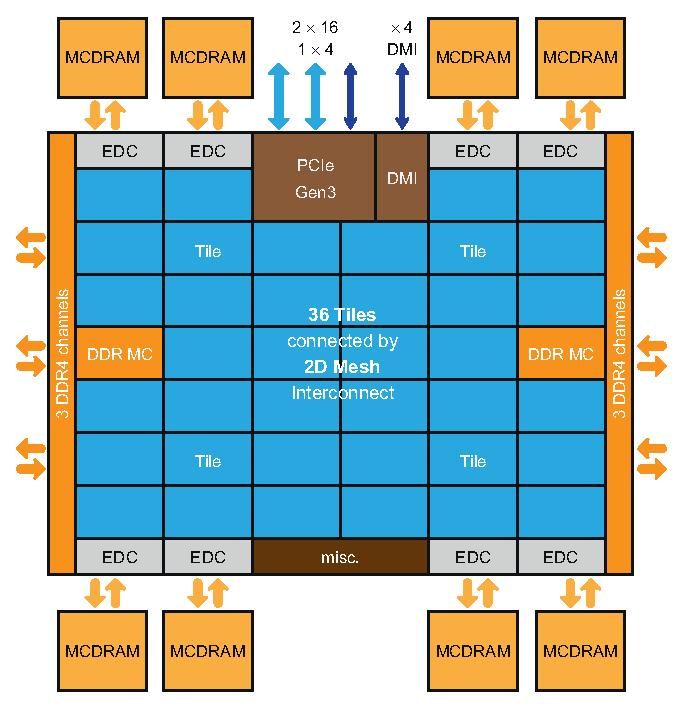
\includegraphics[width=0.7\textwidth]{knl.eps}
        \end{center}
      \end{column}
      \begin{column}{.5\textwidth}
        \begin{center}
          %\includegraphics[width=0.7\textwidth]{tile.png}
        \end{center}
      \end{column}
    \end{columns}
    \vspace{3mm}

    \begin{columns}[T]
      \begin{column}{.5\textwidth}
        \begin{itemize}
          \item up to 72 cores @ 1.5 GHz\\ (3.5 TFLOP/s)
          \item 2D Mesh: 700 GB/s
          \item 8 GB MCDRAM: 450 GB/s
          \item 384 GB DDR-4: 90 GB/s
        \end{itemize}
      \end{column}
      \begin{column}{.5\textwidth}
        \begin{itemize}
          \item 2 cores / 4 VPUs
          \item 512-bit Vector Registers (AVX-512)
          \item 4 hardware hyper-threads
          \item 1 MB shared L2 cache
        \end{itemize}
      \end{column}
    \end{columns}

  \end{frame}

  %%%%%%%%%%%%%%%%%%%%%%%%%%%%%%%%%%%%%%%%%%
  %%%   SLIDE 8
  %%%%%%%%%%%%%%%%%%%%%%%%%%%%%%%%%%%%%%%%%%

  \begin{frame}
    \frametitle{General Programming Implications}

    Three Guidelines...
    \begin{enumerate}
      \item \textbf{Scaling}
      \item \textbf{Vectorisation}
      \item \textbf{Data Locality \& Cache Re-use}
    \end{enumerate}
    \vfill

    ... and how they are implemented in QPhiX
    \begin{enumerate}
      \item \textbf{OpenMP thread scheduling} for lattice traversal
      \item Multi-ISA \textbf{C++ code generator} using Vector Intrinsics
      \item \textbf{Cache blocking} into L2 and \textbf{Structures of Arrays} data layout (\textit{tiles})
    \end{enumerate}
    \vfill

    \textbf{Optimisations in QPhiX-codegen:}\\
    L1 \& L2 software prefetches,
    dimensions of tiles (\texttt{SOALEN}),
    streaming stores, gather/scatter, \dots

  \end{frame}

  %%%%%%%%%%%%%%%%%%%%%%%%%%%%%%%%%%%%%%%%%%
  %%%   SLIDE 9
  %%%%%%%%%%%%%%%%%%%%%%%%%%%%%%%%%%%%%%%%%%

  \begin{frame}
    \frametitle{Data layout \& Cache blocking}

    \begin{itemize}
      \item Elementary vector elements are \textit{Structures of Arrays} (SoA):\\[2mm]
        \texttt{typedef FT FourSpinorBlock[3][4][2][SOALEN];}
        \vfill
        % \pause
      \item \texttt{SOALEN} may be a factor of $\texttt{VECLEN} = \texttt{ngy} * \texttt{SOALEN}$:\\[2mm]
        form \textit{tiles} in X-Y-plane (Xeon Phi SP: $16\times1$, $8\times2$, $4\times4$)
    \end{itemize}
    % \pause

    \vspace{-3mm}
    \begin{columns}[T]
      \begin{column}{.5\textwidth}
        \begin{center}
          \begin{itemize}
            \item Then divide lattice in blocks:\\[2mm]
              \; X: \;\texttt{SOALEN}\\
              \; Y, Z: \;\texttt{By}, \texttt{Bz}\\[2mm]
              such that 3 T-Slices fit into L2
              \vfill
              \vspace{3mm}
            \item Distribute blocks to cores/threads \& process in chunks
              of SIMD vectors, \textit{i.e.} tiles
              \vfill
          \end{itemize}
        \end{center}
      \end{column}
      \begin{column}{.5\textwidth}
        \begin{center}
          %\includegraphics[width=\textwidth]{XYplane.png}
          \vfill
        \end{center}
      \end{column}
    \end{columns}

  \end{frame}

  %%%%%%%%%%%%%%%%%%%%%%%%%%%%%%%%%%%%%%%%%%
  %%%   SLIDE 10
  %%%%%%%%%%%%%%%%%%%%%%%%%%%%%%%%%%%%%%%%%%

  \begin{frame}[fragile]
    \frametitle{QPhiX-codegen}

    \begin{itemize}
      \item Three abstract (class) objects:
        \begin{enumerate}
          \item \texttt{Instruction}: FLOPs, Memory inst., scope delimiters, if-else, \dots
          \item \texttt{Address}: Memory addresses to deal with pointers \& offsets
          \item \texttt{FVec}: ``The registers'' which are fed to intrinsic calls, \textit{i.e.}
            variables in C++ code (\textit{e.g.} of type \texttt{\_\_m512d})
        \end{enumerate}
        % \pause

      \item First two classes: \;\; \texttt{std::string serialize(void)}
      \item Save Instructions into \texttt{InstVector}'s and dumb to file
        % \pause
    \end{itemize}

    \tiny
    %\lstinputlisting[language=C++]{codegen.cc}
\end{frame}

  %%%%%%%%%%%%%%%%%%%%%%%%%%%%%%%%%%%%%%%%%%
  %%%   SLIDE 11
  %%%%%%%%%%%%%%%%%%%%%%%%%%%%%%%%%%%%%%%%%%

  \begin{frame}[fragile]
    \frametitle{Code Example 1: NEW Clover Term Multiplication}
    \tiny

    \begin{columns}[T]
      \begin{column}{.5\textwidth}
        %\lstinputlisting[language=C++]{old.cc}
      \end{column}
      \begin{column}{.5\textwidth}
        %\lstinputlisting[language=C++]{new.cc}
      \end{column}
    \end{columns}
    % \pause

    %\lstinputlisting[language=C++]{clover.cc}
\end{frame}

  %%%%%%%%%%%%%%%%%%%%%%%%%%%%%%%%%%%%%%%%%%
  %%%   SLIDE 12
  %%%%%%%%%%%%%%%%%%%%%%%%%%%%%%%%%%%%%%%%%%

\begin{frame}[fragile]
    \frametitle{Code Example 2: Extending the User Interface}
    \tiny
%\lstinputlisting[language=C++]{user.cc}
\end{frame}


  %%%%%%%%%%%%%%%%%%%%%%%%%%%%%%%%%%%%%%%%%%
  %%%   SLIDE 13
  %%%%%%%%%%%%%%%%%%%%%%%%%%%%%%%%%%%%%%%%%%

  \begin{frame}
    \frametitle{Performance of $A^{-1} \, \slashed D \, x $ Kernels}
    \vspace{-5mm}
    \footnotesize

    \begin{columns}[T]
      \begin{column}{.5\textwidth}
        \begin{center}
          $c_{sw} = 0, \; \mu = 0$ \\
          %\includegraphics[width=0.8\textwidth]{wils_32.png}
          \vfill
          $c_{sw} \neq 0, \; \mu = 0$ \\
          %\includegraphics[width=0.8\textwidth]{clov_32.png}
          \vfill
        \end{center}
      \end{column}
      \begin{column}{.5\textwidth}
        \begin{center}
          $c_{sw} = 0, \; \mu \neq 0$ \\
          %\includegraphics[width=0.8\textwidth]{twmd_32.png}
          \vfill
          $c_{sw} \neq 0, \; \mu \neq 0$ \\
          %\includegraphics[width=0.8\textwidth]{twmc_32.png}
          \vfill
        \end{center}
      \end{column}
    \end{columns}

  \end{frame}

  %%%%%%%%%%%%%%%%%%%%%%%%%%%%%%%%%%%%%%%%%%
  %%%   SLIDE 14
  %%%%%%%%%%%%%%%%%%%%%%%%%%%%%%%%%%%%%%%%%%

  \begin{frame}
    \frametitle{Optimisation Features on KNC vs. KNL}
    \footnotesize

    {\tiny
    Displayed is the basic \textit{dslash} stencil ($c_{sw}=\mu=0$) in single precision
    with $\texttt{SOA}=16$.}

    \begin{columns}[T]
      \begin{column}{.5\textwidth}
        \begin{center}
          KNC:\\
          %\includegraphics[width=1.0\textwidth]{wils_knc_old.png}
          \vfill
        \end{center}
      \end{column}
      \begin{column}{.5\textwidth}
        \begin{center}
          KNL:\\
          %\includegraphics[width=1.0\textwidth]{wils_knl_old.png}
          \vfill
        \end{center}
      \end{column}
    \end{columns}

    \begin{itemize}
      \item KNL natively supports prefetches \& streaming stores much better than KNC
        \vfill
      \item Visible benefits from data layout tuning (shown here: SoA length tuning)
        \vfill
      % \item greatest benefits from algorithmic improvements
    \end{itemize}

  \end{frame}

  %%%%%%%%%%%%%%%%%%%%%%%%%%%%%%%%%%%%%%%%%%
  %%%   SLIDE 15
  %%%%%%%%%%%%%%%%%%%%%%%%%%%%%%%%%%%%%%%%%%

  \begin{frame}
    \frametitle{Multi-node results}
    \footnotesize

    \begin{columns}[T]
      \begin{column}{.5\textwidth}
        \begin{center}
          Dual-Socket Xeon (Haswell):\\
          %\includegraphics[width=1.0\textwidth]{multi_xeon.png}
          \vfill
        \end{center}
      \end{column}
      \begin{column}{.5\textwidth}
        \begin{center}
          Xeon Phi (KNC):\\
          %\includegraphics[width=1.0\textwidth]{multi_knc.png}
          \vfill
        \end{center}
      \end{column}
    \end{columns}

    \bigskip

    \begin{itemize}
      \item STRONG scaling up to 64 Xeon / 16 KNC nodes for various volumes
        \vfill
      \item WEAK scaling up to 64 KNC nodes
        \vfill
    \end{itemize}

  \end{frame}

  %%%%%%%%%%%%%%%%%%%%%%%%%%%%%%%%%%%%%%%%%%
  %%%   SLIDE 16
  %%%%%%%%%%%%%%%%%%%%%%%%%%%%%%%%%%%%%%%%%%

  \begin{frame}
    \frametitle{Conclusions \& Outlook}

    \begin{itemize}
      \item Added new data type \& dynamic memory allocation facilities
      \item Implemented low-level Twisted-Mass-Clover kernels \& hardware feature utility functions
      \item Extended User Interface, added Testing \& Timing for new kernels,
        expanded autoconf/automake setup \dots
      \item Confirmed performance expectations on single KNL's processors
        \vspace{5mm}
        \pause
      \item Interface for tmLQCD
      \item Non-degenerate Twisted-Mass/Twisted-Mass-Clover \textit{dslash}
      \item Twisted boundary conditions
      \item New Algorithms: Domain decomposition, Multi-grid, \dots ?
        \vfill
    \end{itemize}
    \pause

  \end{frame}

  %%%%%%%%%%%%%%%%%%%%%%%%%%%%%%%%%%%%%%%%%%
  %%%   6. BACK UP
  %%%%%%%%%%%%%%%%%%%%%%%%%%%%%%%%%%%%%%%%%%

  % \begin{frame}
  %   \centering
  %   \Large
  %   Back-up slides
  % \end{frame}

% \begin{frame}[fragile]
  %   \frametitle{Integrating Twisted Mass into the Code Generator}

  %   \begin{itemize}
  %     \item Have to store clover terms as two full blocks
  %   \end{itemize}

  %   \begin{columns}[T]
  %     \begin{column}{.5\textwidth}
  %       \lstinputlisting[language=C++]{old.cc}
  %     \end{column}
  %     \begin{column}{.5\textwidth}
  %       \lstinputlisting[language=C++]{new.cc}
  %     \end{column}
  %   \end{columns}

  %   \begin{itemize}
  %     \item Define new \texttt{Address} \& \texttt{FVec} classes for declarations, loads \& prefetches
  %       to L1 and L2 caches
  %   \end{itemize}

  %   \lstinputlisting[language=C++]{pref.cc}
% \end{frame}


  \begin{frame}
      \frametitle{Single Node Performance}

      \centering
      \begin{tikzpicture}
          \begin{axis}[
                  xmin = 1.5,
                  xmax = 3.5,
                  xtick={2, 3},
                  xticklabels={4, 8},
                  xlabel={SoA length},
                  ylabel={GFlop/s},
                  ybar,
                  legend pos=outer north east,
                  ymajorgrids=true,
              ]

              \addplot+[error bars/.cd, y dir=both, y explicit] coordinates {( 2.0 , 166.009833333 ) +- (0, 2.27407204467 ) ( 3.0 , 276.273916667 ) +- (0, 1.93651624652 ) };
              \addlegendentry{ HALF }
              \addplot+[error bars/.cd, y dir=both, y explicit] coordinates {( 2.0 , 191.19375 ) +- (0, 6.59475283119 ) ( 3.0 , 243.890916667 ) +- (0, 2.48770228507 ) };
              \addlegendentry{ SINGLE }
              \addplot+[error bars/.cd, y dir=both, y explicit] coordinates {( 2.0 , 113.832583333 ) +- (0, 0.551468890257 ) ( 3.0 , 109.738241667 ) +- (0, 2.46219177387 ) };
              \addlegendentry{ DOUBLE }

          \end{axis}
      \end{tikzpicture}
  \end{frame}

  \begin{frame}
      \frametitle{Multi Node Performance}
      \framesubtitle{Parameters}

      \begin{itemize}
          \item SOALEN = 8
          \item Block size = 4
          \item Single precision
          \item 12-Parameter gauge compression
          \item Lattice sizes $32^3 \times 64$, $48^3 \times 96$, and $64^3 \times 128$
      \end{itemize}

      \begin{itemize}
          \item Cache mode
          \item Quadrant configuration
          \item One MPI rank per KNL
          \item 8, 16, 32, and 64 KNL
          \item Different rank geometries ($g_1 g_2 g_3 g_4 = \text{\# ranks}$)
      \end{itemize}
      
  \end{frame}

  \begin{frame}
      \frametitle{Multi Node Performance}
      \framesubtitle{Strong Scaling}

      \centering
      \begin{tikzpicture}
          \begin{axis}[
                  xmin=0,
                  ymin=0,
                  xlabel={Number of Nodes},
                  ylabel={GFlop/s Total},
                  legend pos=outer north east,
                  grid=major,
              ]
              \addplot+[only marks, mark=+, error bars/.cd, y dir=both, y explicit]
              table[y error index=2] {strong-64.tsv};
              \addlegendentry{$L = 64$}
              \addplot+[only marks, mark=+, error bars/.cd, y dir=both, y explicit]
              table[y error index=2] {strong-48.tsv};
              \addlegendentry{$L = 48$}
              \addplot+[only marks, mark=+, error bars/.cd, y dir=both, y explicit]
              table[y error index=2] {strong-32.tsv};
              \addlegendentry{$L = 32$}
          \end{axis}
      \end{tikzpicture}
  \end{frame}

  \begin{frame}
      \frametitle{Multi Node Performance}
      \framesubtitle{Lattice Size Scaling}

      \centering
      \begin{tikzpicture}
          \begin{axis}[
                  xlabel={Linear Lattice Size $L$},
                  ylabel={GFlop/s Total},
                  legend pos=outer north east,
                  grid=major,
              ]

              \addplot+[only marks, mark=+, error bars/.cd, y dir=both, y explicit]
              table[y error index=2] {weak-64.tsv};
              \addlegendentry{64 Nodes}

              \addplot+[only marks, mark=+, error bars/.cd, y dir=both, y explicit]
              table[y error index=2] {weak-32.tsv};
              \addlegendentry{32 Nodes}

              \addplot+[only marks, mark=+, error bars/.cd, y dir=both, y explicit]
              table[y error index=2] {weak-16.tsv};
              \addlegendentry{16 Nodes}

              \addplot+[only marks, mark=+, error bars/.cd, y dir=both, y explicit]
              table[y error index=2] {weak-8.tsv};
              \addlegendentry{\phantom 1 8 Nodes}

          \end{axis}
      \end{tikzpicture}
  \end{frame}

  \begin{frame}
    \titlepage
  \end{frame}

  \end{document}
